\documentclass[runningheads]{llncs}
% lmodern: without it, [T1]{fontenc} falls back to Type 3 bitmap EC fonts on any
% TeX Live lacking cm-super, and the body text ships as unsearchable bitmaps.
\usepackage{lmodern}
\usepackage[T1]{fontenc}
\usepackage[utf8]{inputenc}
\usepackage{graphicx}
\usepackage{array}
% Text extracted from the PDF is what the manuscript verifier reads, so how the
% fonts map back to Unicode matters here beyond cosmetics. Measured on this build:
% cmap makes EN-DASHES extract correctly on this build (verified: "0.46--0.53"
% comes back as "0.46-0.53" and the PDF carries 24 en-dash characters). That is
% the one that could corrupt a claim: without it a stated range merges into a
% single wrong number. LIGATURES are NOT fixed: the T1
% encoding still emits fi/fl/ff as single glyphs that pdftotext returns as C0
% control bytes, so "finding" extracts as "nding". The verifier compensates for
% that with its own T1_LIGATURES table; do not read this line as a claim that
% extraction is clean.
\usepackage{cmap}
% The Markdown captions carry their own "Table 1:" / "Figure 2:" labels, and the
% in-text references point at those numbers. LaTeX's float counters number in
% placement order, which is not the same order, so letting both run produced
% captions reading "Table 1. Table 1:" and "Fig. 3. Figure 1:". Suppress the
% automatic label and let the manuscript's own numbering stand.
\usepackage{caption}
\captionsetup{labelformat=empty,labelsep=none}
\usepackage{booktabs}
\usepackage{needspace}
\usepackage{amsmath}
\usepackage[hidelinks,pdftitle={When the Benchmark Answers Itself: Predicate-Defined Relevance and the Limits of Query Understanding in Pharmaceutical Quality-Event Retrieval},pdfauthor={Phani Kumar Balagam},pdfsubject={predicate-defined relevance, retrieval benchmark, pharmaceutical quality, evaluation circularity},pdfcreator={scripts/10\string_build\string_latex.py}]{hyperref}
\usepackage{orcidlink}
\usepackage[expansion=false]{microtype}
\renewcommand{\UrlFont}{\ttfamily\small}
% xurl lets a long URL break at any character. Without it the FDA guidance URL in
% the bibliography ran about 4.7cm past the right margin.
\usepackage{xurl}
% Long \texttt tokens (file paths, model ids) are single unbreakable words to TeX
% and overhang the margin. [htt]{hyphenat} was tried and withdrawn: it breaks them
% by inserting a REAL hyphen, so "results/retrieval_results.json" rendered as
% "re-sults/..." across a line break and a reader cannot tell the hyphen is not
% part of the path. \seqsplit breaks at any character without inserting one, which
% is the same property xurl gives URLs. inline() inserts \allowbreak after each
% "/" and "_" in a long \texttt token, which breaks without adding a character.
\emergencystretch=2em

\begin{document}

\title{When the Benchmark Answers Itself: Predicate-Defined Relevance and the Limits of Query Understanding in Pharmaceutical Quality-Event Retrieval}
\titlerunning{When the Benchmark Answers Itself}
\author{Phani Kumar Balagam\orcidlink{0009-0007-6762-399X}}
\authorrunning{P. K. Balagam}
\institute{Independent Researcher, United States\\
\email{balagam.phani@gmail.com}\\
\url{https://github.com/phanibalagam}}

\maketitle

\begin{abstract}
We release QUEST-QI, a benchmark for evidence retrieval over pharmaceutical quality events and, to our knowledge, the first public one in this domain: 171 questions from six templates yielding 15 distinct stems, with gold sets defined by executable predicates over structured fields. We report two results that point in opposite directions. First, a diagnosis: eight retrievers, including a pretrained BGE encoder and a fusion that uses it, span 0.136--0.341 nDCG@10, and the best overall of them scores 0.193, 0.151, 0.161 and 0.024 on the four question families carrying defect semantics --- the last effectively zero because no document contains the phrase a geography-constrained question uses. The pretrained encoder alone (0.288 micro, 0.296 macro) is statistically indistinguishable from corpus-trained fusion (0.302 micro, 0.280 macro), and the two aggregates disagree on which leads. Second, a null we cannot resolve at this sample size: the only query-understanding component we could build that infers its slot rather than reading it off, an unsupervised defect-category centroid prior, recovers +0.014 nDCG@10 (95\% CI [$-$0.005, 0.033], Holm p = 0.304). We also show why the obvious stronger result is not a retrieval result. Adding that prior to a filter over the metadata a question names reaches 0.579 (the soft metadata filter alone reaches 0.423; a hard prefilter with no defect prior reaches 0.464), but the filter re-executes the gold predicate: a control adding a constant to every gold document, over the same 300-document pool, reaches 0.823, and the answer key 1.000. The configuration recovers about half of what that control is worth (0.53, 95\% CI [0.31, 0.72]), and none of it is retrieval. Any benchmark whose relevance is defined by an executable predicate rewards systems for reconstructing it; we quantify how much on this one.
\keywords{predicate-defined relevance, retrieval benchmark, pharmaceutical quality, evaluation circularity}
\end{abstract}


\section*{Disclaimer}
This work was carried out independently, on personal time and equipment, and is not connected to the author's employment. The views expressed are the author's own and do not represent the views, positions or policies of any current, former or future employer or client. No proprietary, confidential or internal data of any organization was used. All data is public: the openFDA drug enforcement bulk export (US federal public domain, export date 2026-08-27), and two pretrained sentence encoders downloaded from their public repositories with their commit hashes recorded.


\section{Introduction}
A pharmaceutical quality investigation begins with a question about precedent. An investigator holding a new deviation asks whether the same failure mode has been seen before in the same dosage form, whether it has ever been classified as a serious hazard, whether it clusters in a particular period or manufacturing geography, and what the same firm has on record. The answers shape root-cause hypotheses, CAPA scope and effectiveness-check design, and they must be traceable to source records because a regulator will ask where each statement came from.

Retrieval-augmented generation \cite{lewis2020rag} is the obvious architecture, and the obvious build is to embed the records, retrieve the nearest neighbours of the question, and let a language model write the answer with citations \cite{gao2023alce}. We find that this fails on precisely the questions investigators ask. A question about sterility assurance in injectables retrieves records about sterility assurance in tablets; a question about events outside the United States retrieves nothing relevant at all, because no record says ``outside the United States''.

That much is a clean empirical finding. The rest of this paper is about what we could not then demonstrate. The natural next step is to represent the question's structure, parsing out the defect mode, the severity class, the period and the geography, and use it to rank. Doing so raises nDCG@10 from 0.302 to 0.579. But that number is not a retrieval result. Our structured filter compares the same fields, with the same regular expressions, that the benchmark used to define which documents are relevant; the filter \textit{is} the relevance function. We size the problem with controls that do no query understanding at all and simply score documents by gold membership: additively over our 300-document candidate pool such a control reaches 0.823, and ranking the gold set first reaches 1.000. Our best configuration recovers about half of the first of those. When we strip out everything that re-executes the predicate, the remainder, an unsupervised defect-category prior, is worth +0.014 nDCG@10, with a confidence interval spanning zero. That remainder is an upper bound rather than a clean measurement: the prior matches against the same stored \texttt{defect\_category} field the gold rule tests, so even it is not fully independent of the predicate (Section 5.3).

We report this because the failure mode generalises. Predicate-defined relevance is attractive for building benchmarks without an annotation budget, and this paper is a worked example of how it silently converts a retrieval evaluation into a test of predicate reconstruction.

\textbf{Contributions.}

\begin{enumerate}
\item \textbf{QUEST-QI}: 4,652 recall events from the openFDA drug enforcement export, a 15-class defect taxonomy, and 171 investigator-style questions generated automatically from six templates whose slot fillers yield 15 distinct question stems, with gold evidence sets defined by executable predicates over structured fields, split into dev (52) and test (119). The questions are not human-written and the gold sets are not adjudicated; Section 7 states what that costs.
\item \textbf{A distantly-supervised defect taxonomy} labeling 96.1\% of events from canonical phrases in the FDA reason-for-recall field, with a classifier for the free-text tail cross-validated at 0.717 macro F1 overall and 0.609 on the rule-free subset that resembles the tail it is actually applied to.
\item \textbf{A diagnosis} of where text-only retrieval fails, tested against a pretrained encoder rather than asserted: the best text-only system answers entity questions at 0.796 nDCG@10 and defect-semantics questions at 0.151--0.193, falling to 0.024 when the question constrains geography. Adding BGE to the fusion moves that family from 0.000 to 0.024, which is to say nowhere. Corpus-trained and pretrained representations are indistinguishable overall, and which one leads depends on whether the aggregate is taken over queries or over families.
\item \textbf{An inconclusive null and its measurement}: the query-understanding component that infers its slot from the question recovers +0.014 nDCG@10 (CI [$-$0.005, 0.033]); the configuration that reads slots off the question recovers +0.277, which is about half of what a gold-membership control over the same candidate pool is worth, together with the pool-size and scoring-mechanism sensitivities of that fraction.
\end{enumerate}


\section{Related work}
\textbf{Retrieval-augmented generation and its evaluation.} RAG couples a retriever to a generator so that answers can be attributed to non-parametric memory \cite{lewis2020rag,gao2023ragsurvey}. Evaluation has followed two lines. One measures attribution directly, asking whether each generated statement is supported by the cited passage \cite{rashkin2021attribution,bohnet2022aqa,gao2023alce,min2023factscore}. The other automates end-to-end judgement with a second language model \cite{es2023ragas,saadfalcon2023ares,zheng2023llmjudge}. Both lines presuppose that the retrieved passages are the right ones; surveys of hallucination \cite{ji2022hallucination} and of trustworthy RAG \cite{ni2025trustworthyrag} identify retrieval failure as an upstream cause of unsupported generation. This paper evaluates only the retrieval stage, and reports that in this domain it is the binding constraint.

\textbf{Where the retrieval literature places the difficulty.} Benchmarks such as BEIR \cite{thakur2021beir} and studies of RAG robustness \cite{chen2023benchmarkingrag} treat the retriever as the component to improve, and the dominant response has been better document representations: dense passage retrieval \cite{karpukhin2020dpr}, contrastive pre-training \cite{izacard2021contriever,wang2022e5} and the benchmarks that rank them \cite{muennighoff2022mteb}. A smaller line rewrites the query instead, generating a hypothetical answer to retrieve against \cite{gao2022hyde} or letting the model decide when and what to retrieve \cite{asai2023selfrag}. Our diagnosis motivates the second line. On this corpus the spread across document representations is 0.205 nDCG@10 across eight systems, and the pretrained retrieval encoder among them is statistically indistinguishable from corpus-trained fusion here, while giving a system the query's defect category is worth 0.107 on top of the corpus-trained fusion, and 0.069 more than the strongest system in that spread reaches on its own --- an oracle over one component of the gold predicate, not an obtainable signal (Section 5.4). But our attempt to exploit that asymmetry produced a null, and the apparent success we first measured was an artifact of benchmark construction. Position effects in long contexts \cite{liu2023lostinmiddle} are downstream of everything here.

\textbf{Benchmark construction and its biases.} That test collections encode biases which flatter some systems over others is an old and well-established result, and our finding is a special case of it rather than a new phenomenon. Zobel showed that pooled collections are incomplete in ways that systematically disadvantage systems absent from the pool \cite{zobel1998reliable}, and Buckley and Voorhees quantified how incompleteness changes measured ordering \cite{buckley2004incomplete}; Buckley et al. named the limits of pooling for large collections directly \cite{buckley2007bias}. Fuhr catalogued the evaluation errors that follow when these properties are ignored \cite{fuhr2017mistakes}.

Automatically generated collections trade annotation cost for exactly this risk. Azzopardi and de Rijke showed that simulated known-item queries carry a bias determined by the generation procedure \cite{azzopardi2007simulated}; pseudo test collections built from anchor text or from microblog structure inherit the biases of the signal used to build them \cite{asadi2011pseudo,berendsen2013pseudo}, and weak supervision derived from an existing ranker teaches a model that ranker's behavior \cite{dehghani2017weak}. Dietz et al. survey the general case of human-optional collections \cite{dietz2020humansoptional}, and Rahmani et al. examine the same question for collections generated by language models \cite{rahmani2024synthetic}. The parallel outside IR is annotation artifacts: models reach high accuracy on NLI and fact-verification benchmarks by exploiting regularities introduced during dataset construction rather than by performing the task \cite{gururangan2018artifacts,schuster2019fever}.

What we add is not the observation but a measurement recipe. Where the relevance rule is an executable predicate, the rule can itself be run as a ranking signal, and doing so turns an abstract worry into a number on the same scale as the leaderboard. Our contribution is that this control needs two choices stated together, not one: how the gold signal enters the score, and what candidate set it can reach. Getting either wrong moves the number by more than any system in our Table 2 (Section 5.1), and the second choice is the one the literature above does not force an author to declare.

\textbf{Domain applications.} Language models encode substantial clinical knowledge \cite{singhal2022clinicalknowledge}, but recall records are operational documents rather than textbook knowledge, and a corpus that extends to 2026 sits at or beyond current models' knowledge horizon. To our knowledge no public benchmark exists for retrieval over pharmaceutical quality and manufacturing records; the openFDA enforcement data \cite{openfda_enforcement} has been used for epidemiological description rather than as a retrieval corpus.


\section{QUEST-QI}

\subsection{Corpus}
We use the official openFDA drug enforcement bulk export (public domain, export date 2026-08-27), containing 17,899 records. A record is a product line; a recall \textit{event} can span hundreds of product lines sharing one firm, one reason for recall and one classification. An investigator reasons about events, so we aggregate by \texttt{event\_id}, which also removes duplication that would otherwise dominate every metric, since one event in this export spans 470 records.

The corpus holds \textbf{4,652 events} from 1,655 firms in 24 countries, spanning 2012--2026 (mean 3.85 records per event, median 1, max 470). By classification: 2,911 Class II, 1,142 Class III, 598 Class I, 1 not yet classified. Each event becomes one retrieval document containing firm, location, classification, status, initiation and report dates, the reason-for-recall text, up to eight distinct product presentations, distribution pattern and notification mode; documents average 117 words (median 93, p95 263).


\subsection{A defect taxonomy from canonical phrases}
The FDA reason-for-recall field usually opens with a canonical defect phrase terminated by a delimiter, as in ``CGMP Deviations:'', ``Lack of Assurance of Sterility;'' or "Labeling

\begin{itemize}
\item ...". We exploit this in three tiers. \textbf{Prefix tier}: the leading phrase is matched
\end{itemize}

against an ordered rule set of 15 categories (3,615 events). \textbf{Short tier}: the reason has no delimiter but is short enough ($\leq$60 characters) to be a canonical phrase itself, and matches the same rules (855 events). \textbf{Classifier tier}: free-text narratives, labeled by a TF-IDF logistic regression (182 events, 3.9\%).

Rules cover \textbf{96.1\%} of the corpus. The classifier trains \textit{only} on prefix-tier events and \textit{only} on the text following the canonical phrase (3,559 examples), so the seed evidence is never a feature. Five-fold cross-validation gives \textbf{0.717 macro F1} and 0.783 micro F1, but that figure flatters the tail. 64.4\% of those remainders still contain a phrase that some rule matches, and 34.1\% still echo the rule that produced their own label. Restricted to the 1,266 remainders where no rule fires, which is the population the classifier actually faces, macro F1 is \textbf{0.609} (micro 0.728). We treat the rule-free figure as the estimate that matches deployment. Figure 1 shows the category distribution alongside the per-category scores.


\begin{figure}[t]
\centering
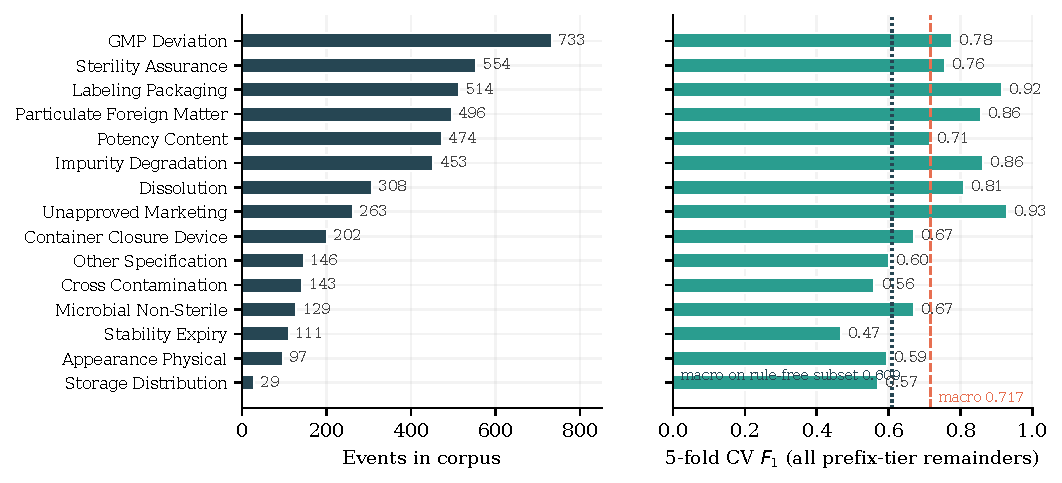
\includegraphics[width=\linewidth]{figures/fig1_taxonomy.pdf}
\caption{Figure 1: The 15-category defect taxonomy. Left, events per category. Right, five-fold cross-validated F1 on the phrase-stripped task; the dashed line is overall macro F1 (0.717), which overstates performance on the free-text tail by about 0.11.}
\end{figure}

Well-separated categories are unapproved marketing (0.93), labeling and packaging (0.92) and impurity/degradation (0.86). Weak ones are stability/expiry (0.47) and cross-contamination (0.56), both sharing vocabulary with neighbours.


\subsection{Benchmark construction}
Each query pairs a natural-language question with a structured predicate; the gold evidence set is every corpus event satisfying that predicate. This removes human relevance judgement from the benchmark and makes it reproducible from the corpus alone. Table 1 gives the six families with an example of each; Section 5.4 shows what the arrangement costs.

The questions are \textbf{generated, not written}. One template per family is instantiated with slot fillers drawn from the taxonomy, the severity classes, the dosage-form vocabulary, the firm list and the period grid. The 171 questions are all distinct as strings, but they reduce to 15 distinct 45-character stems, and within a family the variation is confined to the slots. Two consequences follow and we do not hide either. Lexical diversity is far below what an investigator population would produce, so the absolute levels in Table 2 should not be read as an estimate of live performance. And because a template pairs one phrasing with one predicate, a system that learned the template-to-predicate map would score well without understanding anything; Section 5.4 is in part a measurement of how much of that map our own systems recovered. No human adjudicated any query--document pair. Section 7 records this as the benchmark's principal limitation and states what an adjudicated version would require.


\begin{table}[t]
\centering
\small
\caption{Table 1: The six question families, their predicates and one generated example each. Every question in the benchmark is an instantiation of one of these six templates; the 15 distinct question stems are the slot fillers applied to them.}
\begin{tabular}{lrp{0.52\linewidth}}
\toprule
Family & Predicate & Example question \\
\midrule
A & defect $\times$ dosage form & \textit{Find previous recall events for sterile injectable products where sterility of the finished product could not be assured.} \\
B & defect $\times$ severity class & \textit{Which recalls with the most serious health consequences (Class I) were driven by a situation where the amount of active ingredient was outside the labeled strength?} \\
C & firm & \textit{Summarize every recall event on record for the firm Amneal Pharmaceuticals, LLC.} \\
D & defect $\times$ period & \textit{Between 2019 and 2021, which recalls happened because the batch did not meet its release testing profile for drug release rate?} \\
E & defect $\times$ non-US geography & \textit{Find recalls from firms located outside the United States where a degradant or impurity exceeded its acceptance criterion.} \\
F & site country & \textit{What recall events involve product manufactured or recalled from a site in Spain?} \\
\bottomrule
\end{tabular}
\end{table}

Questions use investigator phrasing and deliberately avoid the FDA canonical phrase, so no system can succeed by string-matching a category name: the STERILITY\_ASSURANCE category is asked as ``sterility of the finished product could not be assured'', never as ``Lack of Assurance of Sterility''.

Family D's predicate uses the recall \textit{initiation} year rather than the FDA report year, which differ for 14.4\% of events. The choice aligns the predicate with the field the metadata filter reads, so that the two are not silently measuring different things. It gives text-only systems no lexical advantage: both dates are written into the document text, but as unsegmented eight-digit tokens (\texttt{20190315}), which the tokeniser keeps whole, so neither date is matchable against ``Between 2019 and 2021'' by any of our lexical channels.

We keep queries whose gold set holds 3--75 events and sample up to 45 per family with a fixed seed, giving \textbf{171 queries} (3,646 query--event gold pairs over 2,185 distinct events; gold set size median 15, mean 21.3, max 71). A stratified 30/70 split yields \textbf{52 dev and 119 test} queries. $\lambda$, the only swept hyper-parameter, is chosen on dev; every headline number is reported on test.


\section{Systems}
All systems index the 4,652 event documents and rank on one CPU core, with no external API and no data leaving the boundary. That is a design choice, adopted because it is what an on-premise deployment in a regulated organization would look like, and not a restriction we were operating under; we say so because the difference matters when reading the Limitations. The pretrained encoders are the single exception: their weights are downloaded once and then run locally, which is what such a deployment would also do.

\textbf{Text channels.} \textit{BM25} \cite{robertson2009bm25}. \textit{TF-IDF} cosine over 1--2-grams with sublinear term frequency. \textit{LSA}, truncated SVD to 300 dimensions over the TF-IDF matrix. \textit{word2vec}, skip-gram trained on the corpus (200 dimensions, window 8, 8 epochs), documents as IDF-weighted mean token vectors.

\textbf{Pretrained encoders.} \textit{BGE}, \texttt{BAAI/bge-base-en-v1.5} (768 dimensions, 512-token window), encoded with the asymmetric query instruction it was trained with; \textit{MiniLM}, \texttt{all-MiniLM-L6-v2} (384 dimensions) \cite{reimers2019sbert}. Both are L2-normalized and ranked by inner product. Model commit hashes are recorded in \texttt{results/dense\_\allowbreak{}manifest.json}, so ``we used BGE'' is a checkable statement rather than a model name.

\textbf{Fusion.} \textit{Hybrid RRF}, reciprocal rank fusion (k = 60) of BM25 and LSA. \textit{Hybrid RRF + BGE} additionally fuses the BGE ranking. Hybrid RRF, not the dense fusion, remains the base that every system in Sections 5.3--5.5 is built on and contrasted against, because it is the strongest configuration that needs no downloaded weights and so is the one a reader can reproduce offline. Section 5.3 re-runs the headline contrast on the dense fusion so that nothing turns on this choice.

\textbf{Defect-prior channel} adds one term to the fused score: a prior over the taxonomy, inferred from the question, added to the RRF score of every candidate in the matching category and weighted by $\lambda$.

\begin{itemize}
\item \textit{Classifier prior}: the Section 3.2 classifier applied zero-shot to the
\end{itemize}

question. Deployable, but trained on recall narratives rather than questions.

\begin{itemize}
\item \textit{Centroid prior}: cosine between the question's LSA vector and each category's
\end{itemize}

mean LSA vector, softmax-scaled. Deployable and needs no labeled question data.

Both priors match against the document's \texttt{defect\_category} label, which is the same field the gold predicate tests for families A, B, D and E. They differ from the metadata channel in that the \textit{query} side is inferred rather than read off the question, imperfectly, at 31\% and 58.3\% top-1 accuracy, and the document side is a label derivable from the document's own text. We describe them as inferring the slot, not as independent of the predicate.

\textbf{Metadata channel} reads severity class, year range, country and dosage form from the question by pattern and down-weights violating candidates by 0.5 (\textit{soft metadata filter}) or removes them before ranking (\textit{metadata prefilter}). \textbf{This channel re-executes the benchmark's gold predicate}; Section 5.4 treats it as a measurement of circularity rather than as a system.

\textbf{Gold-membership lookup} down-weights every document outside the gold set by the same factor. It is not a system; it is the control that bounds what the metadata channel can be measuring.

$\lambda$ is chosen per configuration on dev from {0, 0.25, 0.5, 1, 2, 4, 8, 16}; selected values were 0.25 (classifier prior), 2 (centroid), 2 (oracle category), 4 (classifier + metadata), 8 (centroid + metadata) and 4 (oracle + metadata). The additive gold control of Section 5.4 has its constant chosen the same way, on dev, and lands on 4; its dev curve is flat from $\lambda$ = 4 upward (0.8489 at $\lambda$ = 2, then 0.8519 at 4, 8 and 16), because past that point it already ranks every gold document in the pool first. Other settings (the 0.5 down-weight, the centroid softmax temperature of 8, the 300-document candidate pool, RRF k = 60, SVD dimension 300 and the 3--75 gold-size window) were fixed a priori and never swept; they are recorded in \texttt{results/proposed\_\allowbreak{}results.json} under \texttt{unswept\_hyperparameters}. At the selected $\lambda$ the prior term can exceed the maximum achievable RRF score, so the constrained configurations are better described as ranking by predicted category and tie-breaking by text than as a balanced fusion.

\textbf{Statistics.} Queries built from the same defect category share most of their gold events, so an i.i.d. bootstrap over queries understates variance. Headline confidence intervals and all contrasts use a cluster bootstrap over 50 clusters: one per defect category, plus one per query for the entity families, whose gold sets are near-disjoint \textit{within} the entity block. Clusters are gold-disjoint within each block, but 44.9\% of the gold events in entity clusters also appear in some defect cluster, so the two blocks are not independent of each other and the intervals are not fully conservative. Note also that the 84 defect-family test queries occupy only 15 clusters, so contrasts driven by those families have an effective n nearer 15 than 119. Resamples are 2,000, drawn once and reused for every statistic, so that two estimates of the same quantity cannot differ by Monte-Carlo noise. Per-family intervals in the result files are i.i.d. over at most 31 queries and should be read as indicative only. Contrasts against the text-only baseline are Holm-corrected within each script's family of comparisons: seven in script 04 (every other system in Table 2 against Hybrid RRF) and eight in script 05 (the eight systems under test; the classifier prior with metadata is one of them and appears nowhere in the manuscript, but is kept in the family, which is conservative). The three gold controls of Section 5.4 are contrasted and reported with raw p only. They are diagnostics of the benchmark rather than candidate systems, so a multiple-comparison family over systems is the wrong home for them; all three sit below the bootstrap's resolution floor in any case, so this choice leaves every adjusted p in the manuscript unchanged. The six channel ablations are reported as intervals without p-values and are not corrected. Because the two-sided p is twice the smaller tail, 2,000 resamples cannot resolve below 0.001; a reported 0.0 means p < 0.001 and we never claim more.

\textbf{What the bootstrap does and does not resample.} The clusters are over queries. The corpus, the taxonomy, the templates and the predicates are held fixed in every resample, so every interval in this paper is a statement about query sampling variability alone. None of them carries uncertainty from the corpus draw, from the taxonomy's rule seeds, from the classifier that labels the 3.9\% free-text tail, or from the choice of template phrasings. A different export of the same openFDA data, or a differently-worded template set, could move these numbers by more than the intervals suggest, and nothing here bounds by how much. Read the intervals as the narrowest of the uncertainties present, not as the total.


\section{Experiments}

\subsection{Text-only retrieval}

\begin{table}[t]
\centering
\small
\caption{Table 2: Text-only retrieval, 119 held-out test queries. Micro is the mean over queries; macro is the unweighted mean over the six question families. Intervals are 2,000-resample cluster bootstraps over 50 defect-category clusters, and are wide enough that only the extremes of this table are separated. Hybrid RRF is the base Sections 5.3--5.5 build on, for the reason given in Section 4; Hybrid RRF + BGE is the strongest text-only system we have under both aggregates. Cells are the four-decimal values in \texttt{results/retrieval\_\allowbreak{}results.json} displayed to three; several sit exactly on a half, where either rounding is correct and this table uses both, so read a third-decimal difference of one unit as a display artifact rather than a result.}
\resizebox{\textwidth}{!}{%
\begin{tabular}{lrrrrrrrr}
\toprule
System & R@10 & R@50 & R@100 & P@10 & \textbf{nDCG@10 (micro)} & 95\% CI (cluster) & nDCG@10 (macro) & MRR \\
\midrule
MiniLM (pretrained) & 0.105 & 0.213 & 0.259 & 0.088 & 0.136 & [0.092, 0.201] & 0.124 & 0.256 \\
word2vec (corpus-trained) & 0.147 & 0.244 & 0.286 & 0.103 & 0.159 & [0.105, 0.241] & 0.119 & 0.245 \\
BM25 & 0.221 & 0.342 & 0.389 & 0.164 & 0.236 & [0.169, 0.339] & 0.200 & 0.333 \\
TF-IDF & 0.241 & 0.362 & 0.416 & 0.166 & 0.264 & [0.186, 0.386] & 0.249 & 0.364 \\
BGE-base (pretrained) & 0.239 & 0.380 & 0.436 & 0.201 & 0.288 & [0.215, 0.393] & 0.296 & 0.410 \\
LSA (corpus-trained) & 0.257 & 0.411 & 0.484 & 0.208 & 0.299 & [0.221, 0.415] & 0.257 & 0.412 \\
Hybrid RRF (BM25 + LSA) & 0.260 & 0.396 & 0.457 & 0.211 & 0.302 & [0.225, 0.420] & 0.280 & 0.410 \\
\textbf{Hybrid RRF + BGE} & \textbf{0.284} & \textbf{0.424} & \textbf{0.494} & \textbf{0.229} & \textbf{0.341} & [0.260, 0.463] & \textbf{0.343} & \textbf{0.500} \\
\bottomrule
\end{tabular}
}
\end{table}

Fusion beats BM25 alone (+0.066, CI [0.034, 0.106], Holm p = 0.0) and TF-IDF alone (+0.039, CI [0.004, 0.072], Holm p = 0.099) and is indistinguishable from LSA alone (+0.003, CI [$-$0.024, 0.031], Holm p = 1.0). Averaged word2vec trails everything ($-$0.143 against fusion), and MiniLM is worse still (fusion beats it by +0.167, CI [0.116, 0.244], Holm p = 0.0). A general-purpose symmetric encoder is the wrong tool here.

\textbf{Neither encoder family dominates, and the aggregate decides which one looks better.} Under the micro-average BGE-base reaches 0.288 against 0.302 for BM25 + LSA fusion, a difference of 0.015 with CI [$-$0.047, 0.076] and Holm p = 1.0. Under the macro-average over families the ordering reverses: BGE 0.296 against 0.280. Both differences are inside the interval, so the defensible statement is that the two are indistinguishable on this corpus, not that either wins. The reversal is not noise about a single number, it is a real difference in shape. The micro-average is dominated by the two largest families, and almost all of corpus-trained fusion's advantage sits in one of them: \texttt{C\_firm\_history}, where it reaches 0.759 against BGE's 0.658, on 31 of 119 test queries. It also leads on \texttt{A\_defect\_form} (0.162 against 0.148, n = 31). BGE is ahead on the other four families: B (n = 18), E (n = 10) and F (n = 4) are small, but D is mid-sized at n = 25. A reader who cares about defect-semantics questions should read the macro column; a reader sampling queries in this benchmark's proportions should read the micro column. We report both and claim neither as the headline.

What is not in dispute is complementarity: adding BGE to the fusion is worth +0.038, CI [0.023, 0.057], Holm p = 0.0 under the micro-average --- it is the only pretrained dense channel added to a fusion here, so there is nothing to rank it against --- and the dense fusion is ahead under both aggregates (0.341 micro, 0.343 macro). Recall notices are short, templated regulatory prose whose discriminating content is firm names, product presentations and defect phrases; a corpus-trained representation captures that vocabulary directly, and a general web-and-QA encoder contributes a different and partly disjoint set of hits rather than a uniformly better one.

Indexing is cheap: under a second for BM25, a few seconds for LSA, tens of seconds for word2vec, and about five minutes to encode the corpus once with BGE on CPU. Per-query latency is in the low milliseconds on one CPU core once indexed; exact wall-clock figures vary run to run and are recorded in \texttt{results/retrieval\_\allowbreak{}results.json}.

The absolute numbers are low, which is the subject of the next section.


\subsection{Where text-only retrieval fails}

\begin{figure}[t]
\centering
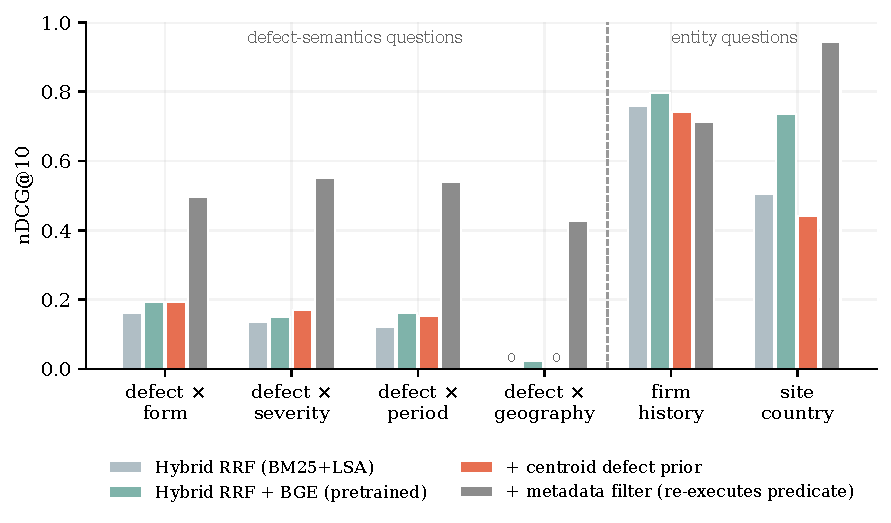
\includegraphics[width=\linewidth]{figures/fig2_family.pdf}
\caption{Figure 2: nDCG@10 by question family, test split. Text-only fusion answers entity questions and collapses on defect-semantics questions. The third bar re-executes the gold predicate and is shown for scale, not as a system.}
\end{figure}

Split by family, the aggregate hides two different regimes. On \textbf{entity questions} (firm history and site country) the best text-only system reaches 0.796 and 0.735 nDCG@10, because the firm or country name is a rare string appearing verbatim in the target documents. On the four \textbf{defect-semantics families} it reaches 0.193, 0.151, 0.161 and \textbf{0.024}.

The last is the clearest case, and it is the one we can now test rather than assert. No document contains ``outside the United States'', so a question built on that constraint retrieves almost nothing relevant. Every lexical channel scores exactly 0.000 on this family; corpus-trained LSA reaches 0.013; \textbf{BGE, a pretrained retrieval encoder, reaches 0.010}, and the fusion that includes it reaches 0.024. Adding a strong pretrained encoder moves this family from nothing to nothing.

The reason is not that the country is missing from the text. It is written down in every document: each opens \texttt{Location: <city>, <state>, <country>}, and 4,462 documents contain the string ``United States''. What no similarity channel can express is the \textit{complement} of that set. Encoding the documents better cannot help, because the operation the question requires is set difference and the operation a similarity score performs is not.

The spread across document representations here is 0.205 nDCG@10 (MiniLM to Hybrid RRF + BGE), and most of it is crossed by corpus-trained channels alone; the pretrained encoder buys the last 0.038. The foot of that spread is itself a pretrained encoder; measuring instead from the weakest corpus-trained channel (word2vec, 0.159), corpus-trained channels still cross 0.143 of the 0.182 that remains above word2vec, 79\% rather than 81\%, so the claim holds under either framing. Giving a system the query's true defect category is worth 0.107 on top of the corpus-trained fusion, and 0.069 more than the strongest system in that spread reaches on its own, for free --- though ``given'' is the operative word: this is an oracle over one component of the gold predicate, not an obtainable signal, and Section 5.4 is about what that distinction costs. That asymmetry is what motivated the rest of this work.

Family sizes on the test split are uneven (A = 31, B = 18, C = 31, D = 25, E = 10, F = 4), so per-family cells carry wide uncertainty, and the pooled aggregate is a mixture weighted by an arbitrary sampling cap. Per-family confidence intervals and the macro-average across families are in \texttt{results/retrieval\_\allowbreak{}results.json}.


\subsection{Query understanding without the predicate}
Figure 3 places every system in this paper on one axis, separating those that infer a constraint from those that read one off the question.


\begin{figure}[t]
\centering
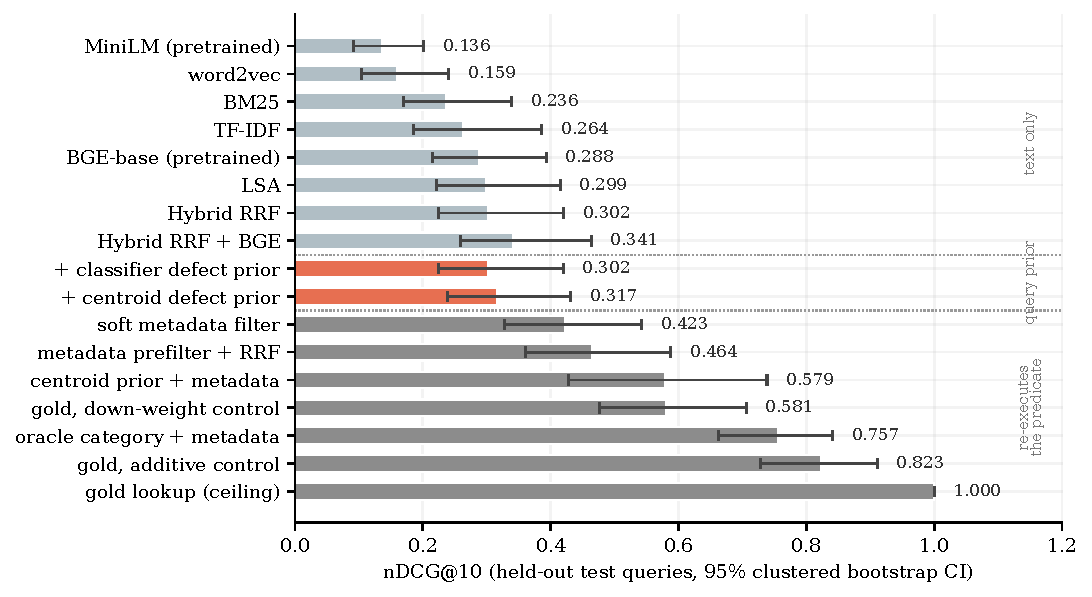
\includegraphics[width=\linewidth]{figures/fig3_main.pdf}
\caption{Figure 3: nDCG@10 on the held-out test split with 95\% clustered bootstrap intervals. Grey, text-only baselines; coral, query-understanding systems that infer the defect category from the question rather than reading a constraint off it; dark grey, configurations that read constraints off the question and so re-execute the gold predicate directly. The coral systems are not predicate-free: they match against the same stored category label the gold rule tests, with a noisy query side, so their gains are upper bounds (Section 5.3).}
\end{figure}


\begin{table}[t]
\centering
\small
\caption{Table 3: Query-understanding systems that infer the defect category from the question alone. Neither reaches significance.}
\resizebox{\textwidth}{!}{%
\begin{tabular}{lrrrrrr}
\toprule
System & R@10 & R@50 & P@10 & \textbf{nDCG@10} & MRR & $\Delta$ vs Hybrid RRF (Holm p) \\
\midrule
Hybrid RRF (text only) & 0.260 & 0.396 & 0.211 & 0.302 & 0.410 & n/a \\
+ classifier defect prior & 0.259 & 0.399 & 0.210 & 0.302 & 0.409 & $-$0.001 [$-$0.007, 0.005] (0.834) \\
+ centroid defect prior & 0.265 & 0.448 & 0.226 & 0.317 & 0.425 & +0.014 [$-$0.005, 0.033] (0.304) \\
\bottomrule
\end{tabular}
}
\end{table}

Table 3 reports both systems. Neither supports the component we set out to build.

\textbf{The supervised query classifier transfers poorly and dev selection all but switches it off.} Applied to the questions it reaches 31\% top-1 category accuracy against a 6.7\% chance rate, far above chance and far below usable. $\lambda$ selected on dev is 0.25, the smallest non-zero value on the grid, and the resulting system is indistinguishable from the text-only baseline ($-$0.001, CI [$-$0.007, 0.005], Holm p = 0.834). A classifier trained on FDA recall narratives does not transfer to investigator phrasing.

\textbf{The unsupervised centroid prior transfers better but does not pay off.} Matching the question against category centroids in the corpus's own LSA space reaches 58.3\% top-1 accuracy, nearly twice the classifier and with no labeled question data, and improves recall@50 from 0.396 to 0.448. But on nDCG@10 it is worth +0.014, CI [$-$0.005, 0.033], Holm p = 0.304. We cannot reject zero.

\textbf{This null is inconclusive, not a demonstration of no effect, and we do not have the sample size to make it one.} The interval runs to +0.033 nDCG@10 at its upper end, an 11\% relative gain over the 0.302 base, comparable to what adding BGE to the fusion buys (+0.038) and half of what fusion over BM25 alone is worth (+0.066). Read as a pair of one-sided tests, the data reject equivalence-to-zero only for margins wider than 0.033, so no equivalence claim at any margin a practitioner would care about is available here. The clustered standard error implied by that interval is about 0.010 nDCG@10; holding the point estimate at +0.014, an interval excluding zero would need roughly twice the query count of the current test split, and more than that after Holm correction. A benchmark of this size cannot settle a +0.014 effect. What we can say is that the centroid prior does not deliver the gain the Section 5.2 asymmetry suggested was available, and that anyone claiming it does needs a larger evaluation than this one.

\textbf{The null is not an artifact of a weak base.} The obvious objection to a null result is that the retriever it sits on top of was too weak to show a gain. We re-ran both priors on the Hybrid RRF + BGE fusion, with $\lambda$ re-selected on dev. The centroid prior is worth +0.020 nDCG@10, CI [0.0002, 0.041], p = 0.048 raw and 0.096 after Holm correction within the pair; the classifier prior is worth +0.001, CI [$-$0.013, 0.015]. The point estimate moves from +0.014 to +0.020 and the interval now barely excludes zero before correction and includes it after. We do not read that as a positive result, and we would not have reported it as one had the dense fusion been our base: it is the same small effect, still not separable from zero at the correction the rest of the paper uses. What it does rule out is the ``your retriever was weak'' reading, because a stronger base makes the defect prior neither redundant nor decisive.

\textbf{Neither prior is fully independent of the predicate, which makes the null stronger.} Both match the question's inferred category against each document's stored \texttt{defect\_category} field, the same field, read from the same file, that the gold rule tests for families A, B, D and E. The query side is inferred rather than parsed, and imperfectly (58.3\% and 31\% top-1), so these are not the metadata channel; but they are soft, noisy partial gold membership rather than a predicate-free signal. This has two consequences. For the 3.9\% of events labeled by classifier rather than rule, the prior and the gold set inherit the \textit{same} model's errors, so the prior is right about them by construction. And the +0.014 is therefore an upper bound on what a genuinely predicate-independent query understanding component would deliver: the predicate-free gain is at most this, and plausibly less. On the four defect-semantics families we have no fully predicate-independent query-understanding system at all; building one would require a category signal derived at query time from document text rather than read from the stored label.

This is the paper's central null, and it is an unresolved one rather than a demonstrated absence. The diagnosis in Section 5.2 says the headroom is in query understanding. Our best attempt at query understanding does not capture it, that attempt was already given a partly circular advantage, and the benchmark is not large enough to distinguish ``does not help'' from ``helps by an amount we cannot see''.


\subsection{What the metadata channel actually measures}
The obvious way to do better is to parse the severity class, period and geography out of the question and filter on them. It works spectacularly and is not a retrieval result.


\begin{table}[t]
\centering
\small
\caption{Table 4: The metadata channel against controls that do no query understanding at all and score documents purely by gold membership. The two control forms differ in how the gold signal enters the score and in whether the 300-document candidate pool is reachable through it. The oracle row is not an independent rung of this ladder: on the four families whose predicate is defect category $\times$ constraint it is numerically identical to the additive control, per family, to every decimal place, because boosting the true category and then penalizing constraint violations selects exactly the gold set. It differs only on the two entity families, where no defect slot exists. The identity is recorded in \texttt{results/proposed\_\allowbreak{}results.json} under \texttt{oracle\_vs\_\allowbreak{}gold\_\allowbreak{}control\_\allowbreak{}by\_family}.}
\begin{tabular}{lrr}
\toprule
Configuration & \textbf{nDCG@10} & $\Delta$ vs Hybrid RRF \\
\midrule
Hybrid RRF (text only) & 0.302 & n/a \\
Soft metadata filter, no defect prior & 0.423 & +0.121 [0.074, 0.166] \\
Hard metadata prefilter + RRF, no defect prior & 0.464 & +0.162 [0.101, 0.221] \\
Centroid prior + metadata filter & 0.579 & +0.277 [0.145, 0.392] \\
Oracle defect category + metadata filter & 0.757 & +0.454 [0.340, 0.540] \\
\textit{Control:} gold membership, down-weight form & 0.581 & +0.278 [0.220, 0.336] \\
\textit{Control:} gold membership, additive form & 0.823 & +0.520 [0.430, 0.594] \\
\textit{Ceiling:} gold ranked first & 1.000 & +0.698 [0.580, 0.775] \\
\bottomrule
\end{tabular}
\end{table}

The benchmark declares an event relevant when \texttt{classification == "Class I"}, when \texttt{year\_from <= init\_\allowbreak{}year <= year\_to}, when \texttt{country == "Spain"}, or when the product text matches a dosage-form regex. The metadata filter tests the same fields with the same comparisons and, for the dosage-form case, the identical regular expression. For family F the filter's accept set \textit{is} the gold set. The one imperfection is family E, where the gold rule requires a non-empty country that is not the United States while the filter only rejects the United States; exactly one corpus event has no country, so the difference is numerically nil. So the question is not whether the metadata configurations reconstruct the predicate, which they do by construction, but how much of the available gain that reconstruction captures.

\textbf{The form of the control matters, and getting it wrong is easy.} Our first control multiplied the score of every non-gold document by the same 0.5 the soft filter uses. It scores 0.581, almost exactly the 0.579 of our best configuration, and we initially read that as proof the configuration had saturated predicate reconstruction. That reading was wrong. A multiplicative down-weight cannot promote a gold document the text channel never surfaced, because zero times a half is zero; it is capped by the text retriever, while the systems it is meant to bound add a constant and can lift documents with no text score at all. Matched to that additive mechanism and the same 300-document candidate pool, the same gold signal reaches \textbf{0.823}, and simply ranking the gold set first reaches \textbf{1.000}.

Taking 0.823 as the denominator, the proposed configuration recovers 53\% of what predicate reconstruction is worth \textit{within the 300-document pool} ((0.579 $-$ 0.302) / (0.823 $-$ 0.302) = 0.532). Three qualifications have to travel with that number, and all three matter.

\textbf{It is not precise.} The fraction is a ratio of two differences, each with a wide interval. Resampling the ratio itself under the same cluster bootstrap gives 95\% CI \textbf{[0.31, 0.72]}. ``Roughly half, between a third and three-quarters'' is as much as the data supports; we use 53\% as shorthand and never as a point estimate.

\textbf{It is not mechanism-matched, by our own standard.} The proposed configuration adds the prior and \textit{then} applies the multiplicative slot penalty (\texttt{s += $\lambda$$\cdot$prior; if violated: s *= 0.5}), so it is additive \textit{and} multiplicative, while the additive control is additive only. The one pairing in this table whose system and control share a mechanism exactly is the purely multiplicative soft filter against the purely multiplicative down-weight control: (0.423 $-$ 0.302)/(0.581 $-$ 0.302) = \textbf{0.434}, CI [0.29, 0.55]. That is the cleanest single statistic here, and it agrees with the headline to within its interval.

\textbf{The middle row measures the candidate pool as much as the mechanism.} Beyond $\lambda$ = 2 the additive control ranks every gold document \textit{in the pool} above every non-gold one, so its score is simply the pool's gold recall and the additive constant stops doing work. \texttt{POOL = 300} was fixed a priori and never swept. Table 5 re-runs both the control and the proposed system at each pool size, with $\lambda$ re-selected on dev for each:


\begin{table}[t]
\centering
\small
\caption{Table 5: The recovered fraction is stable at 0.46--0.53 when both sides see the same pool, but the control's absolute score is not: it is the pool's gold recall and rises to the ceiling as the pool grows.}
\begin{tabular}{lrrr}
\toprule
Candidate pool & Matched control & Proposed & Fraction recovered \\
\midrule
100 & 0.741 & 0.535 & 0.53 \\
300 (reported) & 0.823 & 0.579 & 0.53 \\
600 & 0.894 & 0.600 & 0.50 \\
1,000 & 0.934 & 0.605 & 0.48 \\
2,000 & 0.977 & 0.612 & 0.46 \\
4,652 (full corpus) & 1.000 & 0.628 & 0.47 \\
\bottomrule
\end{tabular}
\end{table}

The fraction survives; the interpretation of the gap between 0.823 and 1.000 does not. That gap is pool truncation rather than scoring mechanism: at full pool the ``mechanism-matched'' control is the literal ceiling. We had presented the two rows as a lesson about matching mechanisms; the fuller lesson is that a gold-membership control measures the reachable candidate set as well as the scoring form, and that both must be stated for the number to mean anything.

Three consequences follow.

First, the +0.277 for the metadata configuration is not evidence about query understanding, and neither is the +0.121 from the constraint channel alone. A conventional filter-then-search system, the kind any engineer would build against a database with no query understanding worth the name, is worth +0.162 nDCG@10 over the same 0.302 baseline --- more than the +0.121 the constraint channel inside the reported configuration is worth on its own. It is a different system rather than a rung on that ladder: it prefilters hard and carries no defect prior. We report the whole ladder rather than the top of it, because the configuration we propose has to clear a system that needs no query understanding at all.

Second, a control of this kind is defined by two choices, not one: how the gold signal enters the score, and what candidate set it can reach. Our first control got the first wrong and was pessimistic by 0.24; reading the second off an unswept constant would have made the same class of error in the other direction. A control reported without both is not interpretable.

Third, this is a general hazard of predicate-defined relevance, not a quirk of our predicates. Any benchmark that declares relevance by an executable rule over document fields will reward a system for reconstructing that rule. Publishing a mechanism-matched gold-membership control and the literal ceiling alongside the leaderboard is cheap and, on this benchmark, decisive.

We keep the metadata numbers in the paper because a reader building such a system should know what filtering buys operationally. We do not claim them as a research result.


\subsection{What would perfect defect-category inference buy?}
A configuration given the true defect category, an oracle over one component of the gold predicate and so subject to the caveat above, reaches 0.410 nDCG@10 without metadata filtering, against 0.317 for the centroid prior and 0.302 for text alone. (With metadata filtering it reaches 0.757, but as Table 4's caption records, that configuration is per-family identical to the gold-membership control on every family where a defect slot exists, so it is a control and not a ceiling on anything.) Read narrowly, that is the ceiling on the category channel \textit{as this benchmark defines categories}: about 0.11 nDCG@10, of which the centroid prior captures 0.014. Read sceptically, it is another measurement of how much of the predicate a system has reconstructed. Both readings support the same conclusion: the category channel is where the remaining headroom sits, and we did not reach it.


\section{Discussion}
\textbf{Report a gold-membership control, and report what defines it.} Any benchmark with predicate-defined relevance should publish, alongside its leaderboard, the score of a system that does no query understanding and ranks purely by gold membership. Section 5.4 is a worked example of how easily that control is mis-specified. It is fixed by two choices, not one: how the gold signal enters the score, and what candidate set it can reach. Getting either wrong moves the number by more than any system in Table 2. Our first attempt was multiplicative and pessimistic by 0.24; the corrected control scores 0.823 against 0.579 for our best configuration, so roughly half the available gain is captured (0.53, CI [0.31, 0.72]; the ratio is of gains over the 0.302 baseline, not of the scores themselves) and none of it is retrieval. Publish the literal ceiling (1.000) alongside it, and state the candidate pool: at full pool the two coincide, which is the clearest evidence that the control's absolute value is a property of the pool. All of it costs a dozen lines of code.

\textbf{The diagnosis survives; the fix is unresolved.} Text retrieval over quality records genuinely fails on defect-semantics questions and genuinely succeeds on entity questions, and neither result depends on the predicate. The questions are paraphrases that never contain the category name, and the failure on geography is a plain absence of the phrase from every document. What we could not show is that a deployable query-understanding component recovers the loss. The unsupervised centroid prior is the most promising direction we tested: it beats a trained classifier by 27 points of category accuracy with no labeled question data, and it does improve recall@50 by 0.05. It is not enough --- though ``not enough'' here means the benchmark could not separate +0.014 from zero, not that the effect is absent; Section 5.3 gives the arithmetic.

\textbf{For a practitioner.} If you are building this system against your own deviation database, filter-then-search is the right first build and will work well. Table 4's 0.464 is real operationally even though it is not a research result. The open problem is the free-text half of the question, where our best attempt bought +0.014. Two cautions on the levels: these questions are template-generated, so real investigator phrasing will be harder than this, and relevance here is a predicate, so these numbers say nothing about how often a system finds what an expert would have wanted.

\textbf{The taxonomy is a reusable artifact.} Rule seeds from canonical phrases, a classifier for the free-text tail, and cross-validation reported on the rule-free subset rather than the flattering aggregate. That procedure transfers to any deviation or CAPA system whose failure-mode field has house conventions.


\section{Limitations}
\textbf{No human adjudicated any relevance judgement, and the questions are generated.} This is the benchmark's principal limitation and it bounds every number in the paper. Gold membership is whatever the predicate returns, so a document a domain expert would call relevant is scored wrong if the predicate excludes it, and vice versa; nothing here estimates how often that happens. The questions are template-generated (Section 3.3), so the lexical variety an investigator population would produce is absent, and a system that learned the template-to-predicate mapping would score well for the wrong reason. Making QUEST-QI a benchmark whose absolute levels can be trusted requires two things we did not do: adjudication of a sample of query--document pairs by at least two qualified reviewers, large enough to estimate agreement with the predicate and with each other; and a set of investigator-written questions, to measure how far the templates distort the difficulty. Until then, read the \textit{contrasts} between systems on this benchmark, which the predicate treats even-handedly, and not the levels.

\textbf{Predicate-defined relevance limits what this benchmark can measure.} Section 5.4 is a limitation as much as a result. QUEST-QI can measure whether a system finds the right documents for questions whose answer is a structured set; it cannot fairly evaluate a system with access to the same structured fields, because such a system can reconstruct the answer key. A version with adjudicated relevance, or with predicates over fields withheld from the ranker, would support claims this one cannot.

\textbf{The category boundaries are the taxonomy's, not an investigator's.} A recall of an oral liquid for black particles in the liquid is labeled PARTICULATE\_FOREIGN\_MATTER, so it is not gold for a question about unmet release specifications, though an investigator would plausibly count it. For the 3.9\% of events labeled by classifier rather than rule, gold membership also inherits that classifier's errors, whose rule-free accuracy is 0.609 macro F1.

\textbf{Recalls are not deviations.} The corpus is public recall records, the visible tail of quality events, written for publication rather than for an investigator. The retrieval findings should transfer, since the questions and their constraint structure are the same, but the taxonomy's phrase conventions are FDA's.

\textbf{One encoder family, no fine-tuning, no reranker.} Table 2 includes a pretrained retrieval encoder, and the diagnosis survives it: BGE-base is indistinguishable from corpus-trained fusion under either aggregate, and geography stays at 0.024. But we tested two encoders from one family at base size, on CPU, with no domain fine-tuning and no cross-encoder reranking stage. A larger or domain-adapted encoder would likely raise Table 2 further, and a reranker would raise it more; neither can express set complement, which is what the geography family requires, so we expect the shape of Figure 2 to hold and the levels to move. Table 2 is a floor, not a ceiling.

\textbf{The encoding step needs network access and a working certificate store.} The encoder weights are downloaded once from huggingface.co and then run entirely locally on CPU; \texttt{scripts/09\_\allowbreak{}dense\_\allowbreak{}encode.py} records each model's commit hash in \texttt{results/dense\_\allowbreak{}manifest.json}, so ``we used BGE'' is a checkable statement. The download is the only step in the pipeline that touches the network, and it failed on our first host for a mundane reason: the Python process did not present the system certificate store, so TLS verification to huggingface.co failed. Injecting it with \texttt{truststore} fixes that, and the script does so. Nothing about this is a property of a regulated deployment, and we do not present it as one.

The practical position for a reader is therefore: the embeddings are regenerable in about six minutes on CPU by running script 09 on any host that can reach huggingface.co with a working certificate store, and the corpus and query ids they are keyed to are checked by scripts 04 and 05, which refuse to run against a stale embedding file. Every other script runs offline, and the pipeline degrades gracefully: without the embedding file, the dense rows and the Section 5.3 robustness check are skipped and everything else is unchanged.

\textbf{Slot extraction is easy by construction, and that is not the main problem.} The templated questions make parsing near-trivial. We flag it, but the circularity in Section 5.4 lies in the \textit{matching}, not the parsing: no parser, however good, would change the conclusion, because the filter compares the same fields the gold rule compares.

\textbf{Dev and test share defect categories and gold documents.} The split is stratified by family, not by defect category: 14 of 15 categories have queries on both sides, and 470 gold events appear in both the dev and the test gold union (dev 895, test 1,760). $\lambda$ is therefore selected on queries whose gold sets overlap those it is evaluated on. We checked the direction: dev selects $\lambda$ = 8 while test is still rising at $\lambda$ = 16, so the leak did not inflate 0.579. It should nonetheless be read as a weaker form of held-out than the phrase usually implies, and a grouped split would be the correct fix.

\textbf{The residual query-understanding result is an upper bound, not a clean measurement.} The centroid and classifier priors match against the stored \texttt{defect\_category} label the gold rule tests (Section 5.3). We report +0.014 as the most predicate-independent number we can produce on this benchmark, not as a predicate-independent number.

Four smaller caveats, recorded for completeness. Test-split family sizes range from 4 to 31, so per-family numbers, especially site-country (n = 4) and geography (n = 10), carry wide uncertainty; intervals are in the result files, and Figure 2 omits them for legibility. Family A's gold matches the dosage-form regex against up to 50 product presentations per event while the document text shows at most eight, so 3.1\% of family-A test gold pairs are invisible to any text system; that is the same class of asymmetry we removed in family D, left in place here because fixing it would change the corpus. The metadata prefilter ranks its whole filtered accept set, while every prior-based system and both gold controls draw from a 300-document pool, which flatters the prefilter relative to the rest of Table 4. And the corpus year range is reported on two different fields: Section 3.1 gives 2012--2026 from report year, initiation years reach back to 2006, and family D's predicate is on initiation year.

\textbf{Human review remains mandatory.} Nothing here is validated for a regulatory context of use. A deployed system built on these components would require qualified human review of every output and the credibility assessment described in \cite{fda_ai_credibility}.


\section{Conclusion}
Retrieval over pharmaceutical quality records fails where investigators need it most: 0.796 nDCG@10 on questions naming a firm, 0.024 on questions constraining manufacturing geography, and a pretrained encoder does not rescue the second. The obvious remedy, representing the question's structure, raises nDCG@10 from 0.302 to 0.579, but a control that does no query understanding and scores documents purely by gold membership reaches 0.823 over the same candidate pool, and ranking the gold set first reaches 1.000. That configuration is therefore recovering about half of what re-executing the benchmark's own relevance rule is worth, and none of it is retrieval. Stripped of everything that reads a constraint off the question, the residual gain from query understanding is +0.014 nDCG@10 with a confidence interval spanning zero. That is an unresolved null rather than a demonstrated absence: the interval also spans a +0.033 gain, which this benchmark is too small to rule out. It is an upper bound besides, because the residual system still matches against the stored field the gold rule tests. We release QUEST-QI, the taxonomy and all scripts at \url{https://github.com/phanibalagam/quest-qi} so the diagnosis can be attacked with better retrievers, and we recommend that any benchmark built on predicate-defined relevance publish a gold-membership control alongside its leaderboard, with both its scoring form and its candidate pool stated.


\needspace{17\baselineskip}
\section*{Reproducibility}
The benchmark, the taxonomy, the scripts below and every file in \texttt{results/} are released at \url{https://github.com/phanibalagam/quest-qi}.

Run in order; each script writes JSON into \texttt{results/}.

\par\noindent\begin{minipage}{\linewidth}
\begin{verbatim}
scripts/01_build_corpus.py     # openFDA export -> 4,652 events
scripts/02_taxonomy.py         # 15-class defect taxonomy + CV
scripts/03_build_benchmark.py  # 171 queries, dev/test split
scripts/09_dense_encode.py     # encoder embeddings (needs network)
scripts/04_retrieval.py        # text-only baselines
scripts/05_taxonomy_aware_retrieval.py   # query understanding + controls
scripts/08_verify_manuscript.py          # re-checks every number here
scripts/10_build_latex.py      # .md -> .tex; --compile builds the PDF
scripts/11_arxiv_package.py    # arXiv source tarball
scripts/12_release_package.py  # repository release archive
figures/gen_figures.py         # all figures, from results/ only
\end{verbatim}
\end{minipage}

Script 09 is the only step that needs network access and the only one that need not be re-run: it writes \texttt{data/processed/\allowbreak{}dense\_\allowbreak{}embeddings.npz}, which scripts 04 and 05 read. Both verify that the embedding file's document and query ids match the current build and refuse to run against a stale one, and both skip their dense channels entirely if it is absent.

Single random seed 20260906 throughout; 2,000 cluster-bootstrap resamples over 50 clusters, drawn once and reused, for all headline intervals and contrasts; Holm correction within each script's family of contrasts against the text-only baseline (seven in script 04, eight in script 05, with the three gold controls contrasted and reported with raw p only, and two more in the Section 5.3 robustness pair). Input data is the openFDA drug enforcement bulk export, public domain, export date 2026-08-27, read from \texttt{data/raw/\allowbreak{}openfda/\allowbreak{}drug\_\allowbreak{}enforcement/} (source URL and SHA-256 in \texttt{data/raw/\allowbreak{}MANIFEST.json}; the resolved path is echoed into \texttt{results/corpus\_\allowbreak{}stats.json}). Dependencies: numpy, scipy, scikit-learn, gensim, rank\_bm25, matplotlib, and, for script 09 only, sentence-transformers. Total runtime a few minutes on one CPU core.

This version is an extended preprint. It runs longer than the 12--15 page limit of a Springer LNCS proceedings paper, and would be cut to a venue's limit before submission; the LNCS class is used here for typesetting only and no venue is claimed.


\section*{Ethics and data statement}
All data is public-domain US federal regulatory data about corporate entities; no personal data is involved. No employer names, internal taxonomies, proprietary records or non-public performance results were used at any point. The defect taxonomy is derived from FDA's own published reason-for-recall conventions. Firm names appear in the corpus because they are part of the public record; nothing here should be read as an assessment of any firm's current quality state, and recall records reflect, among other things, differences in reporting and inspection intensity.


\section*{Declaration of generative AI and AI-assisted technologies}
During the preparation of this manuscript, the author used Claude (Anthropic) to support the drafting and editing of manuscript text and the development and revision of analysis code. The author retained sole responsibility for all final decisions concerning the research question, study design, data selection, outcome definitions, analytical methods and experimental controls; independently verified all sources, data and results; executed and validated the analyses; interpreted the findings; reviewed and edited all AI-assisted content; and assumes full responsibility for the accuracy and integrity of the manuscript.


\section*{On the references}
See \texttt{references.bib}. Every entry was retrieved programmatically from the arXiv API, CrossRef, OpenAlex, the ACL Anthology or the publisher's own page and checked at the source for title, first author, venue, year and page range; where a preprint has since appeared at a venue, the version of record is cited and the eprint retained. No reference was written from memory, and no citation in this manuscript is a placeholder.

One entry carries a note recording a disagreement between sources. The publisher's CrossRef deposit for \texttt{robertson2009bm25} gives 4(1--2):1--174, but those are the fields of a different monograph in the same series (Silvestri, \textit{Mining Query Logs}, 10.1561/1500000013); the published article's own citation line reads 3(4):333--389, and FnTIR 3(3) ends at p. 331. An earlier version of this bibliography followed the deposit. Where an aggregator and the printed article disagree on volume and pages, we cite the article.


\bibliographystyle{splncs04}
\bibliography{references}

\end{document}
